\documentclass[10pt]{beamer}
\usetheme[
%%% option passed to the outer theme
%    progressstyle=fixedCircCnt,   % fixedCircCnt, movingCircCnt (moving is deault)
  ]{Feather}
  
% If you want to change the colors of the various elements in the theme, edit and uncomment the following lines

% Change the bar colors:
%\setbeamercolor{Feather}{fg=red!20,bg=red}

% Change the color of the structural elements:
%\setbeamercolor{structure}{fg=red}

% Change the frame title text color:
%\setbeamercolor{frametitle}{fg=blue}

% Change the normal text color background:
%\setbeamercolor{normal text}{fg=black,bg=gray!10}


% INCLUDE PACKAGES
\usepackage[utf8]{inputenc}
\usepackage[spanish]{babel}
\usepackage[T1]{fontenc}
\usepackage{helvet}
\usepackage{pdfpages}
%\usepackage{multimedia}
\usepackage{media9}
\usepackage{subcaption}
%\usepackage{dtklogos}
\usepackage{tikz}
\usetikzlibrary{patterns}
\usetikzlibrary{mindmap,shadows}
\usetikzlibrary{trees}
\usetikzlibrary{decorations.pathreplacing}
\usepackage{comment}
%\usepackage[hidelinks,pdfencoding=auto]{hyperref}
\usepackage{enumerate}
\usepackage{amsmath}
\usepackage{empheq}
\usepackage[most]{tcolorbox}
\usepackage[font=scriptsize,labelfont=bf]{caption}
\usetikzlibrary{spy}
\usetikzlibrary{calc}
\usepackage{pdflscape}
\usepackage{glossaries}

%%%%%%%%% Tables Utilities %%%%%%%%%%%
\usepackage{array}
\usepackage{multirow}
\usepackage{booktabs}
\usepackage{longtable}
\usepackage{tabularx}
\usepackage{multicol}
\usepackage{rotating}
\usepackage{tabularx}
\setlength{\tabcolsep}{10pt}
\newcolumntype{L}[1]{>{\raggedright\let\newline\\\arraybackslash\hspace{0pt}}m{#1}}
\newcolumntype{C}[1]{>{\centering\let\newline\\\arraybackslash\hspace{0pt}}m{#1}}
\newcolumntype{R}[1]{>{\raggedleft\let\newline\\\arraybackslash\hspace{0pt}}m{#1}}
%%%%%%%%%%%%%%%%%%%%%%%%%%%%%%%%%%%%%%


\usetikzlibrary{shapes.geometric}
\usetikzlibrary{arrows.meta,arrows}
% FOOTNOTES
\renewcommand*{\thefootnote}{\arabic{footnote}}

% DEFFINING AND REDEFINING COMMANDS
%% ARROW
\newcommand{\arrowTikz}[1]
{
	\begin{tikzpicture}[rotate=#1]
		\coordinate (initPoint)   at (0,0);
		\coordinate (endingPoint) at (0.5,0);
		\draw [line width=1pt,-{Stealth[length=3pt,width=4pt,inset=0.3pt]}](initPoint)--(endingPoint);
	\end{tikzpicture}
}

%% SECTION AND SUBSECTIONS REFERENCE
\newcommand{\refsec}[1]{section~\ref{#1}}
\newcommand{\refsubsec}[1]{subsecsection~\ref{#1}}

%% SUPER & SUB SCRIPT
\newcommand{\superscript}[1]{\ensuremath{^{\textrm{#1}}}}
\newcommand{\subscript}[1]{\ensuremath{_{\textrm{#1}}}}
%% BOLD ITEM
\newcommand\litem[1]{\item{\bfseries #1\enspace} \\}
%% WRITE A VECTOR IN BOLD
\newcommand{\bvec}[1]{\vec{\mathbf{#1}}}
%% PARTIAL DERIVATIVE
\newcommand{\pdv}[2]{\frac{\partial #1}{\partial #2}}
%% BIGO
\DeclareMathAlphabet{\mathpzc}{OT1}{pzc}{m}{it}
\newcommand{\bigO}[1]{$\mathpzc{O}(#1)$}
%% FOR TABLES
\newfloatcommand{capbtabbox}{table}[][\FBwidth]
%% EARTH SPHERE DRAWING
\newcommand\pgfmathsinandcos[3]{%
	\pgfmathsetmacro#1{sin(#3)}%
	\pgfmathsetmacro#2{cos(#3)}%
}
\newcommand\LongitudePlane[3][current plane]{%
	\pgfmathsinandcos\sinEl\cosEl{#2} % elevation
	\pgfmathsinandcos\sint\cost{#3} % azimuth
	\tikzset{#1/.style={cm={\cost,\sint*\sinEl,0,\cosEl,(0,0)}}}
}
\newcommand\LatitudePlane[3][current plane]{%
	\pgfmathsinandcos\sinEl\cosEl{#2} % elevation
	\pgfmathsinandcos\sint\cost{#3} % latitude
	\pgfmathsetmacro\yshift{\cosEl*\sint}
	\tikzset{#1/.style={cm={\cost,0,0,\cost*\sinEl,(0,\yshift)}}} %
}
\newcommand\DrawLongitudeCircle[2][1]{
	\LongitudePlane{\angEl}{#2}
	\tikzset{current plane/.prefix style={scale=#1}}
	% angle of "visibility"
	\pgfmathsetmacro\angVis{atan(sin(#2)*cos(\angEl)/sin(\angEl))} %
	\draw[current plane] (\angVis:1) arc (\angVis:\angVis+180:1);
	\draw[current plane,dashed] (\angVis-180:1) arc (\angVis-180:\angVis:1);
}
\newcommand\DrawLongitudeCircleRed[2][1]{
	\LongitudePlane{\angEl}{#2}
	\tikzset{current plane/.prefix style={scale=#1}}
	% angle of "visibility"
	\pgfmathsetmacro\angVis{atan(sin(#2)*cos(\angEl)/sin(\angEl))} %
	\draw[current plane, color = red] (\angVis:1) arc (\angVis:\angVis+180:1);
	\draw[current plane,dashed, color = red] (\angVis-180:1) arc (\angVis-180:\angVis:1);
}
\newcommand\DrawLatitudeCircle[2][2]{
	\LatitudePlane{\angEl}{#2}
	\tikzset{current plane/.prefix style={scale=#1}}
	\pgfmathsetmacro\sinVis{sin(#2)/cos(#2)*sin(\angEl)/cos(\angEl)}
	% angle of "visibility"
	\pgfmathsetmacro\angVis{asin(min(1,max(\sinVis,-1)))}
	\draw[current plane] (\angVis:1) arc (\angVis:-\angVis-180:1);
	\draw[current plane,dashed] (180-\angVis:1) arc (180-\angVis:\angVis:1);
}
\newcommand\DrawLatitudeCircleRed[2][2]{
	\LatitudePlane{\angEl}{#2}
	\tikzset{current plane/.prefix style={scale=#1}}
	\pgfmathsetmacro\sinVis{sin(#2)/cos(#2)*sin(\angEl)/cos(\angEl)}
	% angle of "visibility"
	\pgfmathsetmacro\angVis{asin(min(1,max(\sinVis,-1)))}
	\draw[current plane,red] (\angVis:1) arc (\angVis:-\angVis-180:1);
	\draw[current plane,dashed,red] (180-\angVis:1) arc (180-\angVis:\angVis:1);
}

%% CAPTION FOR EQUATION SET
\newcounter{equationset}
\newcommand{\equationset}[1]{% \equationset{<caption>}
	\refstepcounter{equationset}% Step counter
	\noindent\makebox[\linewidth]{Ecuaci\'on~\theequationset: #1}}% Print caption

% INFORMATION IN THE TITLE PAGE

\title[] % [] is optional - is placed on the bottom of the sidebar on every slide
{ % is placed on the title page
      \textbf{Eliminación de ruido espectral basado en redes neuronales}
}

\subtitle[Escuela Politécnica Superior]
{
      \textbf{Escuela Politécnica Superior}
}

\author[Ignazio F.Finazzi]
{      Ignazio F.Finazzi \\
      {}
}

\institute[]
{
      Escuela Politécnica Superior\\
      Universidad Europea Miguel de Cervantes\\
  
  %there must be an empty line above this line - otherwise some unwanted space is added between the university and the country (I do not know why;( )
}

\date{\today}


% GLOSSARY
%% Definitions and acronyms entries

% \newacronym{uav}{UAV}{Unmanned Aerial Vehicle}
% Reference singular: \gls{uav}   --> UAV
% Reference plural:   \glspl{uav} --> UAVs

% The following definitions will go in the main glossary

% Basics
\newacronym{TFM}{TFM}{Trabajo de Fin de Máster}
\newacronym{UEMC}{UEMC}{Universidad Europea Miguel de Cervantes}
\newacronym{TTF}{TTF}{TrueType Font}
\newacronym{OTF}{OTF}{OpenType Font}


%-------------------------------------------------------
% THE BODY OF THE PRESENTATION
%-------------------------------------------------------

\begin{document}
	% COVER-PAGE
	\bgroup
%\setbeamercolor{background canvas}{bg=beamer@headercolor}
\usebackgroundtemplate{}
\begin{frame}[plain,noframenumbering]{}
	\begin{minipage}[t]{\linewidth-2\fboxsep-2\fboxrule}
		\centering
		\vspace{-0.015\paperheight}
		\hspace*{-1.1385\paperwidth}
		\tikzGraphic
	\end{minipage}
	\hspace*{-1.15\SidebarWidth}
	\centering
	\huge
	\begin{minipage}[c][\textheight][c]{\textwidth}
		
		\centering
		
		{\usebeamerfont{institute}\usebeamercolor[bg]{title}\insertinstitute}\vspace*{30pt}
		
		{\usebeamerfont{title}\usebeamercolor[bg]{title}\inserttitle}\vspace*{30pt}
		
		%{\usebeamerfont{subtitle}\usebeamercolor[bg]{subtitle}\insertsubtitle}\vspace*{30pt}
		
		{\usebeamerfont{author}\usebeamercolor[bg]{title}Autor:\insertauthor}\vspace*{1pt}
		
		{\usebeamerfont{author}\usebeamercolor[bg]{title}Tutora: Patricia Jiménez Fernández}\vspace*{30pt}
		
		{\usebeamerfont{date}\usebeamercolor[bg]{title}\insertdate}\vspace*{\baselineskip}
		
	\end{minipage}
\end{frame}
\egroup
	% TABLE OF CONTENTS
	\begin{frame}{Índice}{}
	\scriptsize{
	\tableofcontents}
\end{frame}
	\scriptsize
	% INTRODUCCION
	\section{Introducción}
		\subsection{Definición y objetivos}
			\begin{frame}{Definición y objetivos}
	\begin{block}{\centering \footnotesize Definición y objetivos}
		%\centering
		El desarrollo del trabajo propuesto consiste en el diseño y prototipado de un sistema la eliminación de ruido en conversaciones habladas.
		\begin{itemize}
			\item Ejecución en tiempo real
			\item Eliminación de gran abanico de ruidos
		\end{itemize}
	\end{block}
\end{frame}
		\subsection{Introducción al Procesamiento de señal}
			\begin{frame}{Introducción al procesamiento de señal}
	\begin{block}{\centering \footnotesize Digitalización}
		%\centering
		Proceso mediante el cual, una señal analógica $x_a(t)$ continua en tiempo y valores pasa a una señal digital $x_d(t)$ discreta en tiempo y valores.
	\end{block}
	\begin{figure}[ht!]
		\centering
		\resizebox{\textwidth}{!}{
			\begin{tikzpicture}
			\tikzstyle{box} = [draw,inner sep=7,minimum size=57,line 
			width=1, very thick, draw=black, fill=black!20]
			\tikzstyle{invisible} = [outer sep=0,inner sep=0,minimum size=0]
			\tikzstyle{stealth} = [-stealth]
			\node [box] (v1) at (-1,0.5) {Muestreador};
			\node [box] (v2) at (3.5,0.5) {Cuantizador};
			\node [box] (v3) at (8,0.5) {Codificador};
			\draw [stealth] (v1) edge node [anchor=south] {$x(n)$} (v2);
			\draw [stealth] (v2) edge node [anchor=south] {$x_q(n)$} (v3);
			\node [invisible] (v4) at (-4,0.5) {};
			\draw [stealth] (v4) edge node [anchor=south] {$x_a(t)$} (v1);
			\node [invisible] (v5) at (11,0.5) {};
			\draw [stealth] (v3) edge node [anchor=south] {$110011$} (v5);
			\draw [dashed] (-2.5,2.5) node [invisible] (v6) {} -- (9.5,2.5) node [invisible] {} -- 
			(9.5,-1) node [invisible] {} -- (-2.5,-1) node [invisible] {} -- (v6);
			\node [invisible] at (3.5,2) {Conversor Analógico Digital};
			\end{tikzpicture}
		}      
		\caption{Esquema de la conversión analógico a digital}
	\end{figure}
\end{frame}
\begin{frame}{Introducción al procesamiento de señal. Muestreo I}
	\begin{block}{\centering \footnotesize Digitalización}
		%\centering
		Proceso mediante el cual, una señal analógica $x_a(t)$ continua en tiempo y valores pasa a una señal $x(n)$ discreta en tiempo y continua en valores.
	\end{block}
	\begin{figure}[ht!]
		\centering
		\resizebox{0.6\textwidth}{!}{
			\begin{tikzpicture}
			\tikzstyle{stealth} = [-stealth, thick]
			\tikzstyle{invisible} = [outer sep=0,inner sep=0,minimum size=0]
			\tikzstyle{circle} = [shape=circle, minimum size=0.5cm, draw=black!55]
			\draw (-0.5,1)node[left,font=\tiny] {$y=+1$} -- (9,1);
			\draw (-0.5,-1)node[left,font=\tiny] {$y=-1$} -- (9,-1);
			\draw (-0.5,-0.33)node[left,font=\tiny] {} -- (9,-0.33); 
			\draw (-0.5,0.33)node[left,font=\tiny] {} -- (9,0.33); 
			\foreach \x in {0,0.25,...,2.25}
			{
				\draw (\x*4,-1.5)node [below,font=\tiny,] {\x } -- (\x*4,1.5) ;
			}
			\draw[ultra thick, ] (0,0) node (v5) {} sin (1,1) node (v7) {};
			\draw[ultra thick, ] (1,1) cos (2,0) node (v9) {};
			\draw[ultra thick, ] (2,0) sin (3,-1) node (v11) {};
			\draw[ultra thick, ] (3,-1) cos (4,0) node (v13) {};
			\draw[ultra thick, ] (4,0)  sin (5,1) node (v15) {};
			\draw[ultra thick, ] (5,1) cos (6,0) node (v17) {};
			\draw[ultra thick, ] (6,0) sin (7,-1) node (v19) {};
			\draw[ultra thick, ] (7,-1) cos (8,0) node (v21) {}; 
			\node [invisible] (v1) at (-0.5,-1.5) {};
			\node [invisible] (v2) at (-0.5,2) {amplitud};
			\node [invisible] (v3) at (10,-1.5) {tiempo};
			\draw [stealth] (v1) edge (v2);
			\draw [stealth] (v1) edge (v3);
			\node [circle] at (0,0) {};
			\node [circle] at (1,1) {};
			\node [circle] at (2,0) {};
			\node [circle] at (3,-1) {};
			\node [circle] at (4,0) {};
			\node [circle] at (5,1) {};
			\node [circle] at (6,0) {};
			\node [circle] at (7,-1) {};
			\node [circle] at (8,0) {};
			\node [invisible] (v4) at (0,-1.5) {};
			\node [invisible] (v6) at (1,-1.5) {};
			\node [invisible] (v8) at (2,-1.5) {};
			\node [invisible] (v10) at (3,-1.5) {};
			\node [invisible] (v12) at (4,-1.5) {};
			\node [invisible] (v14) at (5,-1.5) {};
			\node [invisible] (v16) at (6,-1.5) {};
			\node [invisible] (v18) at (7,-1.5) {};
			\node [invisible] (v20) at (8,-1.5) {};
			\draw [stealth] (v4) edge (v5);
			\draw [stealth] (v6) edge (v7);
			\draw [stealth] (v8) edge (v9);
			\draw [stealth] (v10) edge (v11);
			\draw [stealth] (v12) edge (v13);
			\draw [stealth] (v14) edge (v15);
			\draw [stealth] (v16) edge (v17);
			\draw [stealth] (v18) edge (v19);
			\draw [stealth] (v20) edge (v21);
			\end{tikzpicture}
		}      
		\caption{Esquema del muestreo de una señal de 1Hz muestreada a 4 muestras por segundo}
		\label{fig: sample}
	\end{figure}
\end{frame}
\begin{frame}{Introducción al procesamiento de señal. Muestreo II}
	\begin{block}{\centering \footnotesize Teorema de muestreo de Nyquist-Shannon}
		Si la frecuencia más alta contenida en una señal analógica $x_{a}(t)$ es $F_{max}=B$ y la señal se muestrea a una tasa $F_{s}>2F_{max}\equiv 2B$, entonces $x_{a}(t)$ se puede recuperar totalmente a partir de sus muestras mediante la siguiente función de interpolación
		\begin{align}
		g(t)&=\frac{\sin 2\pi Bt}{2\pi Bt} \\ \nonumber
		&\text{Así, }x_{a}(t)\text{ se puede expresar como:} \\ \nonumber
		x_{a}(t)&=\sum _{n=-\infty }^{\infty }x_{a}\left({\frac {n}{F_{s}}}\right)g\left(t-{\frac {n}{F_{s}}}\right)\\ \nonumber
		&\text{donde }x_{a}\left({\frac {n}{F_{s}}}\right)=x_{a}\left(nT\right)\equiv x\left(n\right)\text{ son las muestras de }x_{a}\left(t\right)
		\end{align}
	\end{block}
	\vspace*{-10pt}
	\begin{columns}
		\column[]{0.45\textwidth}
		{
			\begin{figure}[ht!]
				\centering
				\resizebox{0.8\textwidth}{!}{
					\begin{tikzpicture}
					\tikzstyle{invisible} = [outer sep=0,inner sep=0,minimum size=0]
					\tikzstyle{stealth} = [-stealth]
					\node [invisible] (v1) at (0,0) {};
					\node [invisible] (v2) at (0,2) {};
					\node [invisible] (v3) at (4.5,0) {freq};
					\draw [stealth] (v1) edge (v2);
					\draw [stealth] (v1) edge (v3);
					\draw [dashdotted](2.5,2) -- (2.5,-0.2) node[anchor=north]{$\frac{fs}{2}$};
					
					\draw [invisible, dotted](3.7,0) node [circle] {} -- 
					(3.5,0.8) node [circle] {} -- 
					(3.3,0) node [circle] {};
					\draw [draw](3.5,0.1) -- (3.5,-0.1) node[anchor=north]{\scriptsize$\frac{fs}{2} + \Delta f$};
					\draw [invisible](1.7,0) node [circle] {} -- 
					(1.5,0.8) node [circle] {} -- 
					(1.3,0) node [circle] {};
					\draw [draw](1.5,0.1) -- (1.5,-0.1) node[anchor=north]{\scriptsize$\frac{fs}{2} - \Delta f$};
					\draw [invisible, thick, stealth] plot[smooth, tension=.7] coordinates {(3.5,1) (2.5,1.5) (1.5,1)};
					\node [invisible, anchor=south] at (2.5,1.5) {plegado};
					\end{tikzpicture}
				}
				\vspace*{-10pt}
				\caption{Esquema del plegado de una señal con aliasing}
				\label{fig: aliasing_mirror}
			\end{figure}
		}
		\column[]{0.45\textwidth}
		{
			\begin{figure}
				\centering
				\begin{subfigure}[t]{0.5\textwidth}
					\centering
					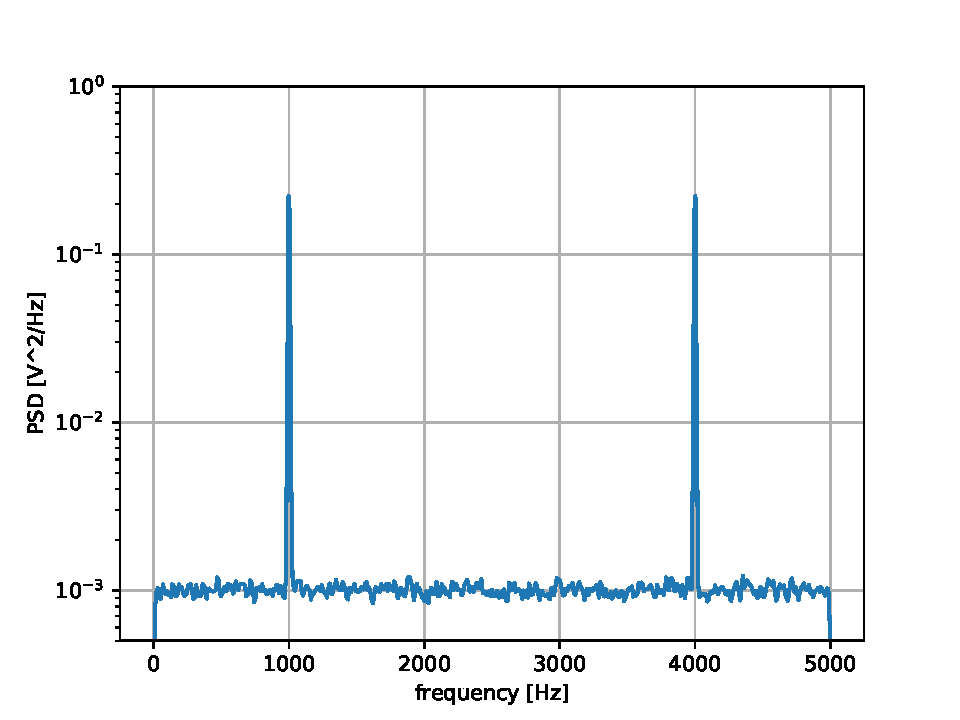
\includegraphics[width=0.9\textwidth]{../figures/pwelch_1k_4k_10k}
					\vspace*{-5pt}
					\caption{Densidad espectral de potencia para la suma dos senos de 1kHz y 4kHz muestreados a 10ksps}
				\end{subfigure}%
				\hspace*{10pt}
				\begin{subfigure}[t]{0.5\textwidth}
					\centering
					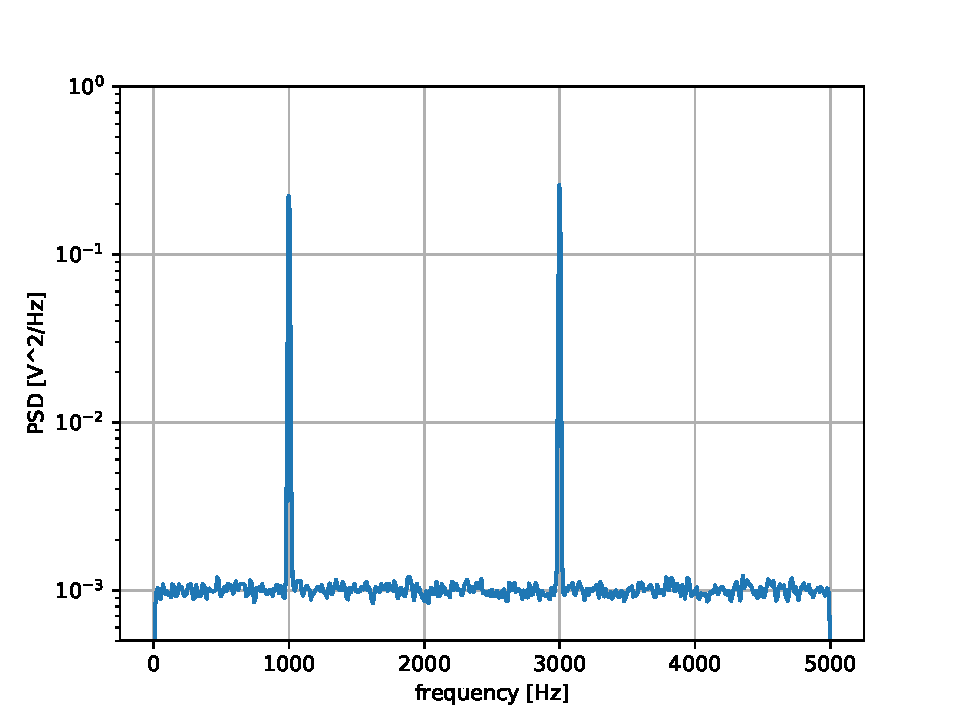
\includegraphics[width=0.9\textwidth]{../figures/pwelch_1k_7k_10k}
					\vspace*{-5pt}
					\caption{Densidad espectral de potencia para la suma dos senos de 1kHz y 7kHz submuestreados a 10ksps}
				\end{subfigure}
				\label{fig: aliasing}
			\end{figure}
		}
	\end{columns}
\end{frame}
\begin{frame}{Introducción al procesamiento de señal. Cuantización}
	\begin{block}{\centering \footnotesize Digitalización}
		%\centering
		Proceso mediante el cual, una señal $x(n)$ discreta en tiempo y continua en valores pasa a una señal digital $x_q(n)$ discreta en tiempo y en valores.
	\end{block}
	\begin{columns}
		\column[]{0.45\textwidth}
		{
			\begin{figure}[ht!]
				\centering
				\resizebox{\textwidth}{!}{
					\begin{tikzpicture}
					\tikzstyle{stealth} = [-stealth, thick]
					\tikzstyle{invisible} = [outer sep=0,inner sep=0,minimum size=0]
					\tikzstyle{circle} = [shape=circle, minimum size=0.5cm, draw=black!55]
					\tikzstyle{line} = [draw, very thick, red]
					\draw (-0.5,1)node[left,font=\tiny] {} -- (10.5,1);
					\draw (-0.5,0.7142)node[left,font=\tiny] {} -- (10.5,0.7142);
					\draw (-0.5,0.4285)node[left,font=\tiny] {} -- (10.5,0.4285);
					\draw (-0.5,0.1428)node[left,font=\tiny] {} -- (10.5,0.1428);
					\draw (-0.5,-0.1428)node[left,font=\tiny] {} -- (10.5,-0.1428);
					\draw (-0.5,-0.4285)node[left,font=\tiny] {} -- (10.5,-0.4285);
					\draw (-0.5,-0.7142)node[left,font=\tiny] {} -- (10.5,-0.7142);
					\draw (-0.5,-1)node[left,font=\tiny] {$y=-1$} -- (10.5,-1);
					\foreach \x in {0,0.1,0.2,0.3,0.4,0.5,0.6,0.7,0.8,0.9,1}
					{
						\draw (\x*10,-1.5)node [below,font=\tiny,] {\x } -- (\x*10,1.5) ;
					}
					\draw[ultra thick, ] (0,0) node (v5) {} sin (2.5,1) node (v7) {};
					\draw[ultra thick, ] (2.5,1) cos (5,0) node (v9) {};
					\draw[ultra thick, ] (5,0) sin (7.5,-1) node (v11) {};
					\draw[ultra thick, ] (7.5,-1) cos (10,0) node (v13) {};
					
					\node [invisible] (v1) at (-0.5,-1.5) {};
					\node [invisible] (v2) at (-0.5,2) {amplitud};
					\node [invisible] (v3) at (11,-1.5) {tiempo};
					\draw [stealth] (v1) edge (v2);
					\draw [stealth] (v1) edge (v3);
					\node [circle] (v4) at (0,0.1428) {};
					\node [circle] (v6) at (1,0.7142) {};
					\node [circle] (v8) at (2,1) {};
					\node [circle] (v10) at (3,1) {};
					\node [circle] (v12) at (4,0.7) {};
					\node [circle] (v14) at (5,0.1) {};
					\node [circle] at (6,-0.7) {};
					\node [circle] (v15) at (7,-1) {};
					\node [circle] at (8,-1) {};
					\node [circle] (v16) at (9,-0.7) {};
					\node [circle] (v17) at (10,0) {};
					\draw [line](0,0.1428) -- (1,0.1428) node [invisible] {} -- (1,0.7) -- 
					(2,0.7) node [invisible] {} -- (2,1) -- 
					(4,1) node [invisible] {} -- (4,0.7) -- 
					(5,0.7) node [invisible] {} -- (5,0.1) node [invisible] {} --
					(6,0.1) -- (6,-0.7) node [invisible] {} --
					(7,-0.7) node [invisible] {} -- (7,-1) -- 
					(9,-1) node [invisible] {} -- (9,-0.7) -- (10,-0.7) -- (10,-0.14);
					\end{tikzpicture}
				}      
				\caption{Esquema de la cuantización con 4 bits a 10 muestras por segundo, i.e., 8 valores posibles}
				\label{fig: cuantization_4bit}
			\end{figure}
		}
		\column[]{0.45\textwidth}
		{
			\begin{figure}[ht!]
				\centering
				\resizebox{\textwidth}{!}{
					\begin{tikzpicture}
					\tikzstyle{stealth} = [-stealth, thick]
					\tikzstyle{invisible} = [outer sep=0,inner sep=0,minimum size=0]
					\tikzstyle{circle} = [shape=circle, minimum size=0.5cm, draw=black!55]
					\tikzstyle{line} = [draw, very thick, red]
					
					\draw (0,0) node [invisible] (v1) {} --
					(4,0) node [invisible] {} --
					(4,4) node [invisible] {} --
					(0,4) node [invisible] {} --
					(0,0) node [invisible] {};
					\foreach \x in {0,0.25,0.5,0.75,1}
					{
						\draw (\x*4,-0.1)node [below,font=\tiny,] {\x } -- (\x*4,0.1) ;
					}
					\foreach \x in {0.125,0.375,0.625,0.875,1}
					{
						\draw (\x*4,-0.1)node [below,font=\tiny,] {} -- (\x*4,0.1);
					}
					\foreach \c [count=\x from 0] in {{000},{001},{010},{011},{100},{101},{110},{111}}
					{
						\draw (-0.1,\x*0.5)node [anchor=east,font=\tiny,] {\c} -- (0.1,\x*0.5);
					}
					%\node at (0,\x) {\c};	
					\draw [line](v1) -- (0.25,0) node [invisible] {} -- 
					(0.25,0.5) node [invisible] {} -- 
					(0.75,0.5) node [invisible] {} -- 
					(0.75,1) node [invisible] {} -- 
					(1.25,1) node [invisible] {} -- 
					(1.25,1.5) node [invisible] {} -- 
					(1.75,1.5) node [invisible] {} -- 
					(1.75,2) node [invisible] {} -- 
					(2.25,2) node [invisible] {} -- 
					(2.25,2.5) node [invisible] {} -- 
					(2.75,2.5) node [invisible] {} -- 
					(2.75,3) node [invisible] {} -- 
					(3.25,3) node [invisible] {} -- 
					(3.25,3.5) node [invisible] {} -- 
					(4,3.5) node [invisible] {};
					\node [invisible] at (2.0187,-1) {$(V_{in}-V_{RefLo})/E_{FSR}$};
					\node [invisible, rotate=90] at (-0.8509,1.9232) {$ADC_{code}$};
					\draw [dashed](0,2) node [invisible] {} -- (2,2) node [invisible] {} -- (2,0) node [invisible] {};
					\draw [dashed](0,3.5) node [invisible] {} -- (3.5,3.5) node [invisible] {} -- (3.5,0) node [invisible] {};
					\draw [dashed](0.25,4) node [] {} -- (0.25,-0.25) node [anchor=north] {\tiny LSB};
					\end{tikzpicture}
				}      
				\caption{Resolución del ADC}
				\label{fig: adc_resolution}
			\end{figure}
		}
	\end{columns}
\end{frame}
		\subsection{Redes LSTM}
			\begin{frame}{Redes recurrentes. Celdas LSTM}
	\begin{columns}
		\column[]{0.45\textwidth}
		{
			\begin{itemize}
				\item Redes \textbf{recurrentes} \arrowTikz{0} Las redes neuronales recurrentes son aquellas que retienen información de sus estados anteriores y ante los mismos estímulos de entrada no siempre producen las mismas salidas, debido al estado de la celda.
			\end{itemize}
		}
		\column[]{0.45\textwidth}
		{
			\begin{figure}[ht!]
				\centering
				\resizebox{0.9\textwidth}{!}{
					\begin{tikzpicture}
					\tikzstyle{box} = [draw,inner sep=7,minimum size=57,line 
					width=1, very thick, draw=black, fill=black!20, text width=60pt, text centered]
					\tikzstyle{stealth} = [-stealth, thick]
					\tikzstyle{invisible} = [outer sep=0,inner sep=0,minimum size=0]
					\tikzstyle{circle} = [shape=circle, minimum size=0.5cm, draw=black!55]
					\tikzstyle{line} = [draw, very thick, red]
					
					\begin{scope}
					\node [box] (v2) at (0,0) {Neurona tradicional};
					\node [circle, fill] (v1) at (0,2.5) {};
					\node [circle, fill] (v3) at (0,-2.5) {};
					\draw [stealth] (v1) edge node[anchor=east] {$x(t)$} (v2);
					\draw [stealth] (v2) edge node[anchor=east] {$y(t)$} (v3);
					\end{scope}
					\begin{scope}[shift={(3.5,0)}]
					\node [box] (v2_1) at (0,0) {Neurona recurrente};
					\node [circle, fill] (v1_1) at (0,2.5) {};
					\node [circle, fill] (v3_1) at (0,-2.5) {};
					\draw [stealth] (v1_1) edge node [anchor=east] {$x(t)$} (v2_1);
					\draw [stealth] (v2_1) edge node [anchor=east] {$y(t)$} (v3_1);
					\end{scope}
					
					\node [invisible, anchor=east] (v5) at (4.75,1.25) {};
					\draw [stealth, in =0, out=0] (v5) edge node[anchor=north west] {$h(t-1)$} (v2_1);
					\node [invisible] (v4) at (2.25,1.25) {};
					\node [] (v6) at (3.5,1.25) {};
					\draw [thick, in =180, out=180] (v2_1) edge (v4);
					\draw [thick] (v4) edge (v6);
					\draw [thick] (v6) edge (v5);
					\end{tikzpicture}
				}      
				\caption{Comparación de neuronas tradicionales con neuronas recurrentes}
				\label{fig: nn_vs_rnn}
			\end{figure}
		}
	\end{columns}
	\begin{itemize}
		\item Celdas LSTM (Long Short-Term Memory)
		\begin{itemize}
			\item \scriptsize{Propuestas por Sepp Hochreiter y Jürgen Schmidhuber en 1997.}
			\item \scriptsize{Evitan el problema de las dependencias a largo plazo.}
		\end{itemize}
	\end{itemize}
	\vspace*{-5pt}
	\begin{figure}[ht!]
		\centering
		\resizebox{0.8\textwidth}{!}{
			\begin{tikzpicture}
			\tikzstyle{box} = [draw,minimum size=15,line width=1, very thick, draw=black, fill=black!30, text centered]
			\tikzstyle{stealth} = [-stealth, thick]
			\tikzstyle{invisible} = [outer sep=0,inner sep=0,minimum size=0]
			\tikzstyle{circle} = [shape=ellipse, minimum size=15pt, draw=black!, text width=15pt, text centered]
			\tikzstyle{circle_op} = [shape=circle, minimum size=0.5cm, draw=black, very thick, fill=black!10]
			\tikzstyle{line} = [draw, very thick, red]
			\begin{scope}
			\node [circle] (v14) at (-2.25,-0.75) {$x_t$};
			\node [box] (v1) at (-1.5,0.5) {$\sigma$};
			\node [box] (v3) at (-0.5,0.5) {$\sigma$};
			\node [box] (v8) at (0.5,0.5) {$\tanh$};
			\node [box] (v6) at (1.5,0.5) {$\sigma$};
			\node [circle_op] (v2) at (-1.5,2.5) {x};
			\node [circle_op] (v4) at (0.5,1.5) {x};
			\node [circle_op] (v5) at (0.5,2.5) {\scriptsize$+$};
			\node [circle_op] (v7) at (2.5,1.25) {x};
			\node [ellipse, draw, very thick, fill=black!10] (v13) at (2.5,2) {$\tanh$};
			\draw [stealth] (v1) edge (v2);
			\draw [stealth,out=90,in=180] (v3) edge (v4);
			\draw [stealth] (v4) edge (v5);
			\draw [stealth,out=90,in=180] (v6) edge (v7);
			\node [invisible] (v11) at (-2,0) {};
			\node [invisible] (v10) at (-0.5,0) {};
			\node [invisible] (v9) at (0.5,0) {};
			\node [invisible] (v12) at (1,0) {};
			\draw [thick] (v8) edge (v4);
			\draw [thick,] (v9) edge (v8);
			\draw [thick] (v10) edge (v3);
			\draw [thick] (v11) edge (v12);
			\draw [thick,out=0,in=270] (v12) edge (v6);
			\draw [thick] (v7) edge (v13);
			\draw [thick] (v2) edge (v5);
			\draw [thick,out=90,in=180] (v14) edge (v11);
			\draw [thick,out=0,in=270] (v11) edge (v1);
			\node [invisible] (v22) at (-2.75,0) {};
			\node [invisible] (v21) at (-2.75,2.5) {};
			\node [invisible] (v17) at (4,2.5) {};
			\node [circle] (v19) at (3.5,4) {$h_t$};
			\node [invisible] (v16) at (4,0) {};
			\node [invisible] (v15) at (3,0) {};
			\draw [stealth] (v15) edge (v16);
			\draw [stealth] (v5) edge (v17);
			\node (v18) at (3.5,2.5) {};
			\draw [stealth] (v18) edge (v19);
			\node [invisible] (v20) at (3.5,0) {};
			\draw [thick] (v20) edge (v18);
			\draw [thick,out=270,in=180] (v7) edge (v15);
			\draw [thick] (v21) edge (v2);
			\draw [thick] (v22) edge (v11);
			\node [invisible] (v23) at (2.5,2.5) {};
			\draw [thick] (v13) edge (v23);
			\draw [rounded corners=2ex] (-2.75,3) rectangle (3.75,-0.25);
			\end{scope}
			\begin{scope}[shift={(6.75,0)}]
			\node [circle] (v14) at (-2.25,-0.75) {$x_{t+1}$};
			\node [box] (v1) at (-1.5,0.5) {$\sigma$};
			\node [box] (v3) at (-0.5,0.5) {$\sigma$};
			\node [box] (v8) at (0.5,0.5) {$\tanh$};
			\node [box] (v6) at (1.5,0.5) {$\sigma$};
			\node [circle_op] (v2) at (-1.5,2.5) {x};
			\node [circle_op] (v4) at (0.5,1.5) {x};
			\node [circle_op] (v5) at (0.5,2.5) {\scriptsize$+$};
			\node [circle_op] (v7) at (2.5,1.25) {x};
			\node [ellipse, draw, very thick, fill=black!10] (v13) at (2.5,2) {$\tanh$};
			\draw [stealth] (v1) edge (v2);
			\draw [stealth,out=90,in=180] (v3) edge (v4);
			\draw [stealth] (v4) edge (v5);
			\draw [stealth,out=90,in=180] (v6) edge (v7);
			\node [invisible] (v11) at (-2,0) {};
			\node [invisible] (v10) at (-0.5,0) {};
			\node [invisible] (v9) at (0.5,0) {};
			\node [invisible] (v12) at (1,0) {};
			\draw [thick] (v8) edge (v4);
			\draw [thick,] (v9) edge (v8);
			\draw [thick] (v10) edge (v3);
			\draw [thick] (v11) edge (v12);
			\draw [thick,out=0,in=270] (v12) edge (v6);
			\draw [thick] (v7) edge (v13);
			\draw [thick] (v2) edge (v5);
			\draw [thick,out=90,in=180] (v14) edge (v11);
			\draw [thick,out=0,in=270] (v11) edge (v1);
			\node [invisible] (v22) at (-2.75,0) {};
			\node [invisible] (v21) at (-2.75,2.5) {};
			\node [invisible] (v17) at (4,2.5) {};
			\node [circle] (v19) at (3.5,4) {$h_{t+1}$};
			\node [invisible] (v16) at (4,0) {};
			\node [invisible] (v15) at (3,0) {};
			\draw [stealth] (v15) edge (v16);
			\draw [stealth] (v5) edge (v17);
			\node (v18) at (3.5,2.5) {};
			\draw [stealth] (v18) edge (v19);
			\node [invisible] (v20) at (3.5,0) {};
			\draw [thick] (v20) edge (v18);
			\draw [thick,out=270,in=180] (v7) edge (v15);
			\draw [thick] (v21) edge (v2);
			\draw [thick] (v22) edge (v11);
			\node [invisible] (v23) at (2.5,2.5) {};
			\draw [thick] (v13) edge (v23);
			\draw [rounded corners=2ex,fill=black!60,opacity=0.8] (-2.75,3) rectangle (3.75,-0.25);
			\end{scope}
			\begin{scope}[shift={(-6.75,0)}]
			\node [circle] (v14) at (-2.25,-0.75) {$x_{t-1}$};
			\node [box] (v1) at (-1.5,0.5) {$\sigma$};
			\node [box] (v3) at (-0.5,0.5) {$\sigma$};
			\node [box] (v8) at (0.5,0.5) {$\tanh$};
			\node [box] (v6) at (1.5,0.5) {$\sigma$};
			\node [circle_op] (v2) at (-1.5,2.5) {x};
			\node [circle_op] (v4) at (0.5,1.5) {x};
			\node [circle_op] (v5) at (0.5,2.5) {\scriptsize$+$};
			\node [circle_op] (v7) at (2.5,1.25) {x};
			\node [ellipse, draw, very thick, fill=black!10] (v13) at (2.5,2) {$\tanh$};
			\draw [stealth] (v1) edge (v2);
			\draw [stealth,out=90,in=180] (v3) edge (v4);
			\draw [stealth] (v4) edge (v5);
			\draw [stealth,out=90,in=180] (v6) edge (v7);
			\node [invisible] (v11) at (-2,0) {};
			\node [invisible] (v10) at (-0.5,0) {};
			\node [invisible] (v9) at (0.5,0) {};
			\node [invisible] (v12) at (1,0) {};
			\draw [thick] (v8) edge (v4);
			\draw [thick,] (v9) edge (v8);
			\draw [thick] (v10) edge (v3);
			\draw [thick] (v11) edge (v12);
			\draw [thick,out=0,in=270] (v12) edge (v6);
			\draw [thick] (v7) edge (v13);
			\draw [thick] (v2) edge (v5);
			\draw [thick,out=90,in=180] (v14) edge (v11);
			\draw [thick,out=0,in=270] (v11) edge (v1);
			\node [invisible] (v22) at (-2.75,0) {};
			\node [invisible] (v21) at (-2.75,2.5) {};
			\node [invisible] (v17) at (4,2.5) {};
			\node [circle] (v19) at (3.5,4) {$h_{t-1}$};
			\node [invisible] (v16) at (4,0) {};
			\node [invisible] (v15) at (3,0) {};
			\draw [stealth] (v15) edge (v16);
			\draw [stealth] (v5) edge (v17);
			\node (v18) at (3.5,2.5) {};
			\draw [stealth] (v18) edge (v19);
			\node [invisible] (v20) at (3.5,0) {};
			\draw [thick] (v20) edge (v18);
			\draw [thick,out=270,in=180] (v7) edge (v15);
			\draw [thick] (v21) edge (v2);
			\draw [thick] (v22) edge (v11);
			\node [invisible] (v23) at (2.5,2.5) {};
			\draw [thick] (v13) edge (v23);
			\draw [rounded corners=2ex,fill=black!60,opacity=0.8] (-2.75,3) rectangle (3.75,-0.25);
			\end{scope}
			\end{tikzpicture}
		}
		\vspace*{-5pt}
		\caption{Celdas LSTM}
		\label{fig: lstm}
	\end{figure}
\end{frame}
		\subsection{Estado del arte}
			\begin{frame}[t]{Estado del Arte}
	\begin{table} [h!]
		\centering
		\resizebox{\textwidth}{!}{%
			\begin{tabular}{C{0.6\textwidth} C{0.4\textwidth}}
				\normalsize{\textbf{Algoritmos dominio público}} & \normalsize{\textbf{Algoritmos privativos}} \\ \bottomrule
			\end{tabular}
		}
	\end{table}
	\begin{columns}
		\begin{column}{0.6\textwidth}
			\centering
			\vspace*{-10pt}
			\begin{figure}[ht!]
				\centering
				\begin{subfigure}[t]{0.45\textwidth}
					\centering
					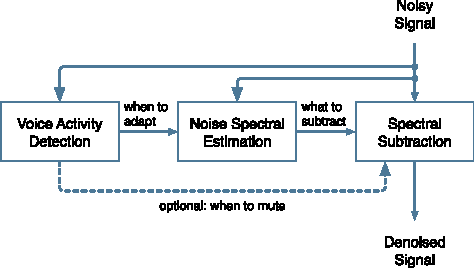
\includegraphics[width=0.9\textwidth]{../figures/rnn_structure.pdf}
					\caption{Estructura del algoritmo presentado por Jean-Marc Valin}
					\label{fig: rnn_structure}
				\end{subfigure}%
				\hspace*{10pt}
				\begin{subfigure}[t]{0.45\textwidth}
					\centering
					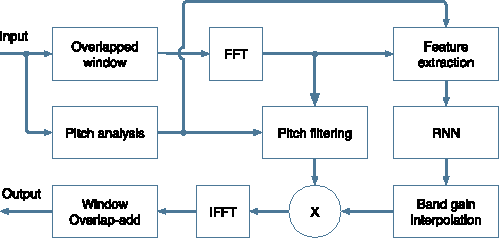
\includegraphics[width=0.9\textwidth]{../figures/rnn_block_diagram.pdf}
					\caption{Diagrama de bloques del eliminación de ruido en el dominio de la frecuencia}
					\label{fig: rnn_block_diagram}
				\end{subfigure}
				\begin{subfigure}[b]{0.65\textwidth}
					\centering
					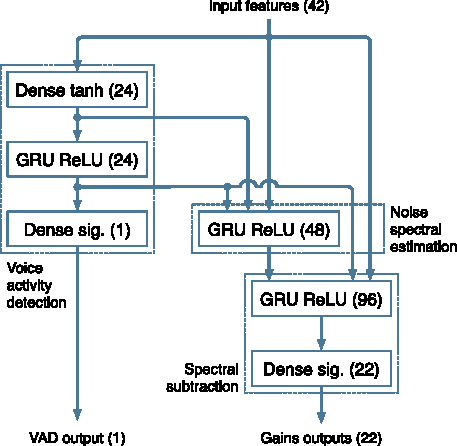
\includegraphics[width=0.9\textwidth]{../figures/rnn_nn.pdf}
					\caption{Red neuronal de RNNoise}
					\label{fig: rnn_nn}
				\end{subfigure}
			\end{figure}
		\end{column}
		\vrule{}
		\begin{column}[t]{0.4\textwidth}
			\vspace*{-100pt}
			\begin{itemize}
				\item \textbf{RTX Voice}
				\begin{itemize}
					\scriptsize
					\item Producto de NVIDIA
					\item \checkTikz{0.2}Gratuito
					\item \redcrossTikz{0.2}Plugins para algunas aplicaciones de chat por voz
					\item \redcrossTikz{0.2}Necesita una gráfica NVIDIA RTX
				\end{itemize}
				\item \textbf{Krisp}
				\begin{itemize}
					\scriptsize
					\item Producto de Krisp
					\item \redcrossTikz{0.2}De pago (gratuito hasta 120$\frac{min}{semana}$)
					\item \checkTikz{0.2}Funciona con el dispositivo de audio del sistema operativo, luego funciona con todo
					\item \checkTikz{0.2}No necesita hardware dedicado
				\end{itemize}
			\end{itemize}
		\end{column}
	\end{columns}
\end{frame}
	% DATA GATHERING
	\section{Obtención, procesado y almacenamiento de datos}
		\subsection{Datos de Audio}
		\subsection{Datos de Ruido}
	% EDA
	\section{Análisis exploratorio de datos}
		\subsection{Análisis de integridad}
		\subsection{Análisis de los datos de audio}
	% MODEL DESIGN
	\section{Diseño e implementación de modelos}
		\subsection{Pre-procesado de datos}
		\subsection{Modelo de capas LSTM}
	% RESULTS
	\section{Análisis de los resultados obtenidos}
	% CONCLUSIONS
	\section{Conclusiones y propuestas de mejora}
	
	% THANKS PAGE
	\bgroup
%\setbeamercolor{background canvas}{bg=beamer@headercolor}
\usebackgroundtemplate{}
\begin{frame}[plain,noframenumbering]{}
	\begin{minipage}[t]{\linewidth-2\fboxsep-2\fboxrule}
		\centering
		\vspace{-0.329\paperheight}
		\hspace*{-1.133\paperwidth}
		\tikzGraphic
	\end{minipage}
	\hspace*{-1.15\SidebarWidth}
	\centering
	\huge
	\ \textcolor{white}{GRACIAS POR SU}
	%\vspace{1 cm}
	\\
	\hspace*{-1.15\SidebarWidth} 
	\textcolor{white}{ATENCIÓN}
	\\
	\vspace*{1 cm}
	\hspace*{-1.15\SidebarWidth}
	%\textcolor{white}{ifinazzi@gte.esi.us.es}
	\vspace*{-2 cm}
\end{frame}
\egroup
\end{document}